\chapter{Clustering}

\section{Evaluation of a new instance}

At this point, with a model trained on the data, a generic $n$th new snapshot instance $\vect{\mathcal{S}}_n$ can be evaluated using the K-means algorithm.
From a geometric point of view, the snapshot $\vect{\mathcal{S}}_n$ is a point in the ${F}$-dimensional space, where ${F}$ is the number of features used to train the model.

For demonstration purposes, in this section, it is considered an example with ${F}=3$ features.

\begin{figure}[htbp]
  \centering
  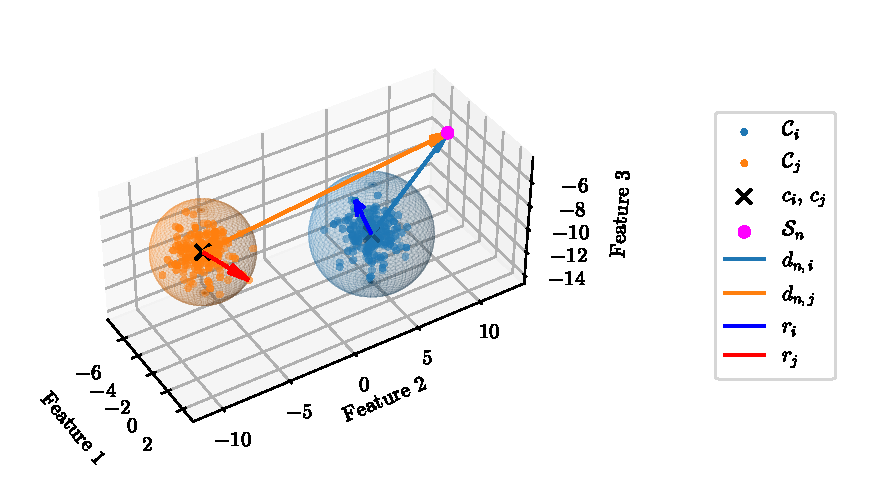
\includegraphics[width=\textwidth]{images/Spheres_2.pdf}
\caption{Cluster model in the $3$-dimensional space, with new snapshot $\vect{\mathcal{S}}_n$}
\label{fig:clust_spheres}
\end{figure}

In the \autoref{fig:clust_spheres}, the training data are represented in the $3$-dimensional space, where the axis are the features used to train the model. The K-means model has been ideally trained with an arbitrary number $k$ of clusters but, for display purposes, only two clusters  ($\vect{\mathcal{C}}_i$ and $\vect{\mathcal{C}}_j$) are plotted. 
\paragraph*{}
The entities shown in the \autoref{fig:clust_spheres} are:
\begin{itemize}
  \item $\vect{\mathcal{C}}_i$ is the set of training snapshots belonging to the $i$th cluster, it has a centroid $\vect{c}_i$ and a radius $\vect{r}_i$;
  \item $\vect{\mathcal{C}}_j$ is the set of training snapshots belonging to the $j$th cluster, it has a centroid $\vect{c}_j$ and a radius $\vect{r}_j$;
  \item $\vect{\mathcal{S}}_n$ is the new snapshot to be evaluated;
  \item $\vect{d}_{n,i}$ is the distance between $\vect{\mathcal{S}}_n$ and $\vect{c}_i$;
  \item $\vect{d}_{n,j}$ is the distance between $\vect{\mathcal{S}}_n$ and $\vect{c}_j$;
\end{itemize}

\subsection{Assign the new instance to a cluster} 
